\documentclass[xcolor=pdftex,table,11pt]{beamer}
\usetheme{Warsaw}
\usepackage[utf8]{inputenc}
\usepackage[english]{babel}
\usepackage{amsmath}
\usepackage{amsfonts}
\usepackage{amssymb}
\usepackage{multirow}
\usepackage{siunitx}
\usepackage{listings}
\usepackage{tabulary}


\usepackage[highlightcolor=yellow]{../styles/code}
\author{Informática I - Instituto Unviersitario Areonáutico}
\title{Introducción a la programación en C}

\usepackage{booktabs}
\usepackage{longtable}
\newcommand*{\thead}[1]{\multicolumn{1}{c}{\bfseries #1}}

\usepackage{tikz}
\def\checkmark{\tikz\fill[scale=0.3](0,.35) -- (.25,0) -- (1,.7) -- (.25,.15) -- cycle;} 

%\setbeamercovered{transparent} 
%\setbeamertemplate{navigation symbols}{} 
%\logo{} 
%\institute{} 
%\date{} 
%\subject{} 
\begin{document}


\begin{frame}
\titlepage
\end{frame}

\begin{frame}
\tableofcontents
\end{frame}






\begin{frame}{Funciones definición}
\begin{block}{}
Las funciones permiten a los desarrolladores dividir un programa en módulos independientes.\\
\begin{itemize}
\item Funciones pre-empaquetadas de C: permiten realizar cálculos matemáticos, operaciones con cadenas de texto, operaciones de entrada y salida de datos, etc.
\item Definidas por el desarrollador: permiten realizar tareas particulares del algoritmo en cuestión.
\end{itemize}

\end{block}

 \begin{figure}
 \centering
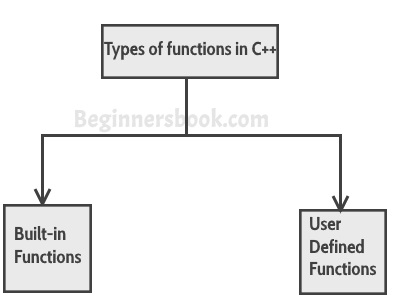
\includegraphics[scale=0.4]{../img/exported/types_of_functions_cpp.jpg}
\end{figure}

\end{frame}



\begin{frame}{Funciones definición}

 \begin{figure}
 \centering
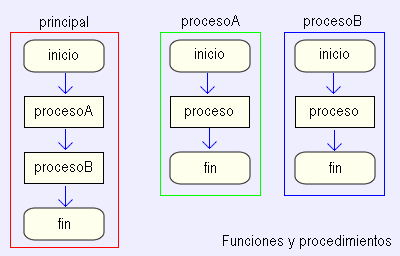
\includegraphics[scale=0.7]{../img/exported/Funciones.png}
\end{figure}

\end{frame}






\begin{frame}[allowframebreaks]{Anatomía de un función en C}
Las funciones se pueden clasificar en 4 tipos según su naturaleza:
\begin{itemize}
\item Si Reciben y si retornan datos: calcular el promedio de dos números
\item No reciben y si retornan datos: menú de opciones
\item No reciben y no retornan datos: función saludo
\item Si reciben y no retornan datos: impresión de datos


\end{itemize}

\end{frame}


\begin{frame}[allowframebreaks]{Anatomía de un función en C}

\begin{block}{Prototipo}
Consiste en una presentación de la función. En el se define que tipo de dato retorna y si lo hace, el nombre de la misma y el tipo de dato de lo/los parámetros que recibe. En caso de ser mas de un parámetros, se los separa por comas.\\
\end{block}

Ejemplos de prototipos:
\codesetstylefrombeamer
\cppfile{../../c/functions/func_prototype.c}


Notar que para indicar que una función no recibe y/o no retorna parámetros, se utiliza la palabra reservada \textbf{void}. Además, las funciones en C pueden recibir muchos valores y de distintos tipos, pero \textbf{sólo pueden retornar un único dato}.

\newpage

\begin{block}{Estructura general de una función en C}
Luego de la declarar el prototipo de la función, se procede a la especificación formal de la misma.
\end{block}





\begin{block}{La sentencia return}
Dicha sentencia fuerza la salida inmediata de la función. Es decir que las sentencias que se encuentren después de una sentencia return(); no serán ejecutadas.\\
Esta sentencia puede ser utilizada para retornar valores, siempre y cuando el tipo de retorno \textbf{no sea void}. 
\end{block}

\newpage
Ejemplo general:
\codesetstylefrombeamer
\cppfile{../../c/functions/func_structure.c}

Ejemplos particulares:


\cppfile{../../c/functions/func_prom.c}

\cppfile{../../c/functions/func_menu.c}


\cppfile{../../c/functions/saludo.c}


\end{frame}

\begin{frame}[allowframebreaks]{Llamada a funciones}
\begin{itemize}
\item  Se realiza con el nombre de la función
\item  Si la función recibe datos, estos deben ser enviados al momento de la llamada. En orden, entre paréntsis y separados por comas
\item  Si la función NO recibe datos, se deben colocar los paréntesis vacíos
\item  Si la función retorna parámetros, debemos asignar el valor de retorno a una variable
\item  Una llamada a una función es una sentencia de C. Por ello debe colocarse el ; al final de la misma

\end{itemize}



\href{https://github.com/danis963/informaticaI_IUA/blob/main/c/src/7-funcion_sumar.c}{\beamergotobutton{Ver ejemplo I completo en github}}


\end{frame}

\begin{frame}{Ámbito de variables}
\begin{block}{Variables locales}

Se declaran dentro de una función y sólo están disponibles durante su ejecución. Cuando la función termina, son destruidas.



\end{block}


\begin{block}{Variables globales}
Globales: Se declaran fuera de las funciones y existen durante todo el ciclo de vida del programa.\\

\textbf{Su uso NO es considerado una buena práctica de programación.}



\end{block}
\href{https://github.com/danis963/informaticaI_IUA/blob/main/c/src/7-variables.c}{\beamergotobutton{Ver ejemplo I completo en github}}


\end{frame}


\begin{frame}[allowframebreaks]{Mecanismo de paso de argumentos a funciones}

\begin{block}{Paso por valor}
El valor del argumento es \textbf{copiado} en el parámetro de la subrutina, por lo cual si se realizan cambios en el mismo dentro de la función, el valor original no es modificado.

\end{block}

\codesetstylefrombeamer

\cppfile{../../c/src/7-paso_por_valor.c}



\begin{block}{Paso referencia}
Se copia la \textit{dirección de memoria} del argumento como parámetro de la función. En este caso, al realizar cambios en parámetro formal este si se ve afectado.
\end{block}
\codesetstylefrombeamer
\cppfile{../../c/src/7-paso_por_referencia.c}


¿Qué significan los símbolos * y \&?


\end{frame}

\begin{frame}[allowframebreaks]{Punteros}
\begin{block}{Definición}
Los punteros son variables cuyos valores son direcciones de memoria. En general, esta dirección de memoria es la ubicación de otra variable.
\end{block}

La declaración de una variable puntero se realiza indicando el tipo de dato, seguido de un * y el nombre de la variable:


\codesetstylefrombeamer
\cppfile{../../c/functions/pointers.c}



\begin{block}{Operador ampersand (\&)}
Se lo conoce como \textit{operador de dirección}. Devuelve la dirección de memoria de un operando.
\end{block}

\begin{block}{Operador *}
Se lo conoce como operador \textit{operador de indirección o desreferencia}, devuelve el valor del objeto al que apunta su operando
\end{block}

Ejemplo:

\codesetstylefrombeamer
\cppfile{../../c/src/9-1-pointers1.c}


 \begin{figure}
 \centering
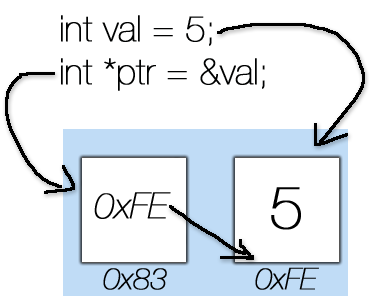
\includegraphics[scale=0.7]{../img/exported/pointers.png}
\end{figure}
\end{frame}

\codesetstylefrombeamer
\cppfile{../../c/src/7-swap.c}

\begin{frame}[allowframebreaks]{Volviendo a las funciones: paso por referencia}
\codesetstylefrombeamer
\cppfile{../../c/src/7-swap.c}
\end{frame}

\begin{frame}[allowframebreaks]{Funciones y arreglos unidimensionales}
\begin{block}{}
A diferencia de las variables en las que podemos elegir pasarlas a una función por valor o referencia, los arreglos sólo se pasan a funciones \textbf{mediante referencia}.\\
Es decir que la función trabajará SIEMPRE con el arreglo original y no con una copia del mismo.
\end{block}


\begin{block}{¿Cómo le indicamos a la función que va a recibir un arreglo?}
Hay tres formas de señalar esto en el prototipo de la función:
\begin{itemize}
\item Como un array con tipo definido y sin dimensiones
\item Como un array con tipo y dimensiones definidas
\item Como un puntero

\end{itemize}


\end{block}
En C/C++ el nombre de un arreglo es un puntero al primer elemento del mismo.


\newpage
Ejemplo utilizando un array con tipo definido y sin dimensiones:
\codesetstylefrombeamer
\cppfile{../../c/functions/func_array_1d.c}

\href{https://github.com/danis963/informaticaI_IUA/blob/main/c/src/7-func_array_1d.c}{\beamergotobutton{Ver ejemplo completo en github}}

\newpage
Ejemplo utilizando un array con tipo y dimensiones definidas:
\codesetstylefrombeamer
\cppfile{../../c/src/7-2func_array_1d.c}

\href{https://github.com/danis963/informaticaI_IUA/blob/main/c/src/7-2func_array_1d.c}{\beamergotobutton{Ver ejemplo completo en github}}



\newpage
Ejemplo utilizando un puntero :) :
\codesetstylefrombeamer
\cppfile{../../c/src/7-3func_array_1d.c}

\href{https://github.com/danis963/informaticaI_IUA/blob/main/c/src/7-3func_array_1d.c}{\beamergotobutton{Ver ejemplo completo en github}}
\end{frame}



\begin{frame}[allowframebreaks]{Ejemplos}
 \begin{enumerate}
   
     \item Diseñar y codificar un programa que implemente las siguientes funciones:
     \begin{itemize}
     \item Saludo: imprimir los datos personales del desarrollador. Prototipo: void saludo(void);
     \item Menú: permitir al operador seleccionar una de las siguientes opciones:
     \begin{itemize}
     \item Cargar un vector de 10 elementos de tipo entero
     \item Imprimir el vector
     \item Imprimir el mayor elemento dentro del arreglo
     \item Imprimir el menor elemento dentro del arreglo
     \item Imprimir la media de todos los elementos del arreglo
	 \item Imprimir los elementos mayores a la media
	 \item Imprimir los elementos menores a la media
     \end{itemize}
     Prototipo: int menu(void);
   
     \item Cargar un vector de 10 elementos de tipo entero.\\
      		Prototipo: void cargar (int []);
	\item Imprimir el vector\\
     Prototipo: void imprimir (int []);

    \item Imprimir el mayor elemento dentro del arreglo. \\
     	     Prototipo: void imprimeMayor (int []);
     	     
      \item Impimir el menor elemento dentro del arreglo\\
     	     Prototipo: void imprimeMenor (int []);
	 
	    \item Imprimir en main la media de todos los elementos del arreglo.\\
    	Prototipo: float calculaMedia (int []);
    	
	 \item Imprimir los elementos mayores a la media, donde la media es recibida como parámetro desde la función main()\\
	  Prototipo: void imprimeMayoresMedia (int [],float);
	  
	  	 \item Imprimir los elementos menores a la media, donde la media es recibida como parámetro desde la función main()\\
	  Prototipo: void imprimeMenoresMedia (int [],float);
     \end{itemize}

\href{https://github.com/danis963/informaticaI_IUA/blob/main/c/src/5-break_cont_1.c}{\beamergotobutton{Ver en github}}


   \end{enumerate}
   
\end{frame}



\begin{frame}[allowframebreaks]{Funciones y arreglos bidimensionales}
\end{frame}
\end{document}